\documentclass[11pt]{article}

% -------------------------
% Packages
% -------------------------
\usepackage[margin=1in]{geometry}
\usepackage{graphicx}
\usepackage{amsmath}
\usepackage{amssymb}
\usepackage{booktabs}
\usepackage{hyperref}
\usepackage{caption}
\usepackage{float}

% -------------------------
% Document
% -------------------------
\begin{document}

% -------------------------
% Title Page
% -------------------------
\begin{titlepage}
    \centering
    \vspace*{2.5cm}

    {\LARGE \textbf{MDR-TS v1.2}}\\[0.5cm]
    {\Large Temporal--Station Baseline for Soil Moisture Prediction}\\[1.5cm]

    {\large Jakob Balkovec}\\[0.3cm]
    {\large Seattle University, Computer Science}\\[0.3cm]
    {\large MDR Project}\\[2cm]

    {\large December 23, 2025}

    \vfill
\end{titlepage}

\section{Executive Summary}

This report summarizes the current state of \textbf{MDR-TS v1.2}, a temporal–station baseline model for soil moisture prediction built using remote sensing, meteorological, and terrain data.

The model is trained on daily time series from \textbf{three in-situ stations} in total: two used for training and validation, and one fully held out for testing. The primary focus of this work is understanding and improving \textbf{spatial generalization} rather than maximizing performance on known stations.

Relative to earlier baseline versions, MDR-TS v1.2 removes calendar and atmospheric shortcut features, specifically day-of-year and relative humidity, which were identified through ablation as harmful to station-level generalization. Removing these features led to lower test error, a shift from negative to positive test $R^2$, and reduced systematic underprediction on the unseen station.

While the model still exhibits residual bias, remaining errors are more consistent with missing temporal memory effects than with feature leakage or model capacity limitations.

\section{Problem Setup and Data}

\subsection{Task Definition}
The task is to predict daily soil moisture at a depth of 5\,cm using remotely sensed and auxiliary environmental variables.

\subsection{Dataset Overview}
All data are sourced from the MDR Temporal Pipeline and consist of daily, station-aligned time series.

\begin{itemize}
\item Training: 2 stations
\item Validation: future time holdout within training stations
\item Test: 1 fully held-out station
\end{itemize}

This split is designed to separate temporal generalization from spatial generalization.

\subsection{Target Variable}
\texttt{soil\_moisture\_5cm}

\subsection{Spatial and Temporal Coverage}
Each station spans multiple years of daily observations. Given the small number of stations, results should be interpreted as directional rather than definitive.

\section{Model Description}

\subsection{Model Choice and Rationale}
An XGBoost regressor is used as a strong and interpretable baseline for tabular data. The model allows for fast iteration and systematic ablation while remaining easy to diagnose.

\subsection{Feature Set (v1.2)}
The retained feature set includes:
\begin{itemize}
\item Meteorological variables: precipitation, air temperature, solar radiation
\item Vegetation indices: NDVI, NDMI, MSI
\item Radar features: Sentinel-1 VV, VH, SAR ratio
\item Terrain attributes: elevation, slope
\end{itemize}

\subsection{Removed Features and Motivation}
The following features were removed based on ablation results:
\begin{itemize}
\item \textbf{Day-of-year (DOY):} introduced a strong seasonal prior that reduced spatial generalization
\item \textbf{Relative humidity:} acted as a station-specific climate proxy and increased bias on unseen stations
\end{itemize}

\section{Experimental Design}

\subsection{Train, Validation, and Test Split Strategy}
Training and validation samples originate from the same stations, with validation performed using future time periods. The test set consists entirely of a held-out station, enabling a clean evaluation of spatial transfer.

\subsection{Evaluation Metrics}
Model performance is evaluated using:
\begin{itemize}
\item Mean Absolute Error (MAE)
\item Root Mean Squared Error (RMSE)
\item Coefficient of Determination ($R^2$)
\item Mean residual (bias)
\end{itemize}

\section{Results}

\subsection{Quantitative Performance Metrics}

\begin{table}[H]
\centering
\begin{tabular}{lccc}
\toprule
Split & MAE & RMSE & $R^2$ \\
\midrule
Train & 0.03198 & 0.04460 & 0.8456 \\
Validation & 0.04696 & 0.06064 & 0.6691 \\
Test & 0.05730 & 0.06840 & 0.2013 \\
\bottomrule
\end{tabular}
\caption{Performance metrics for MDR-TS v1.2}
\end{table}

\subsection{Bias Analysis}
Mean residuals indicate a reduction in systematic underprediction relative to earlier versions:
\begin{itemize}
\item Validation bias: $-0.007$
\item Test bias: $-0.040$
\end{itemize}

\subsection{Diagnostic Plots}

\begin{figure}[H]
\centering
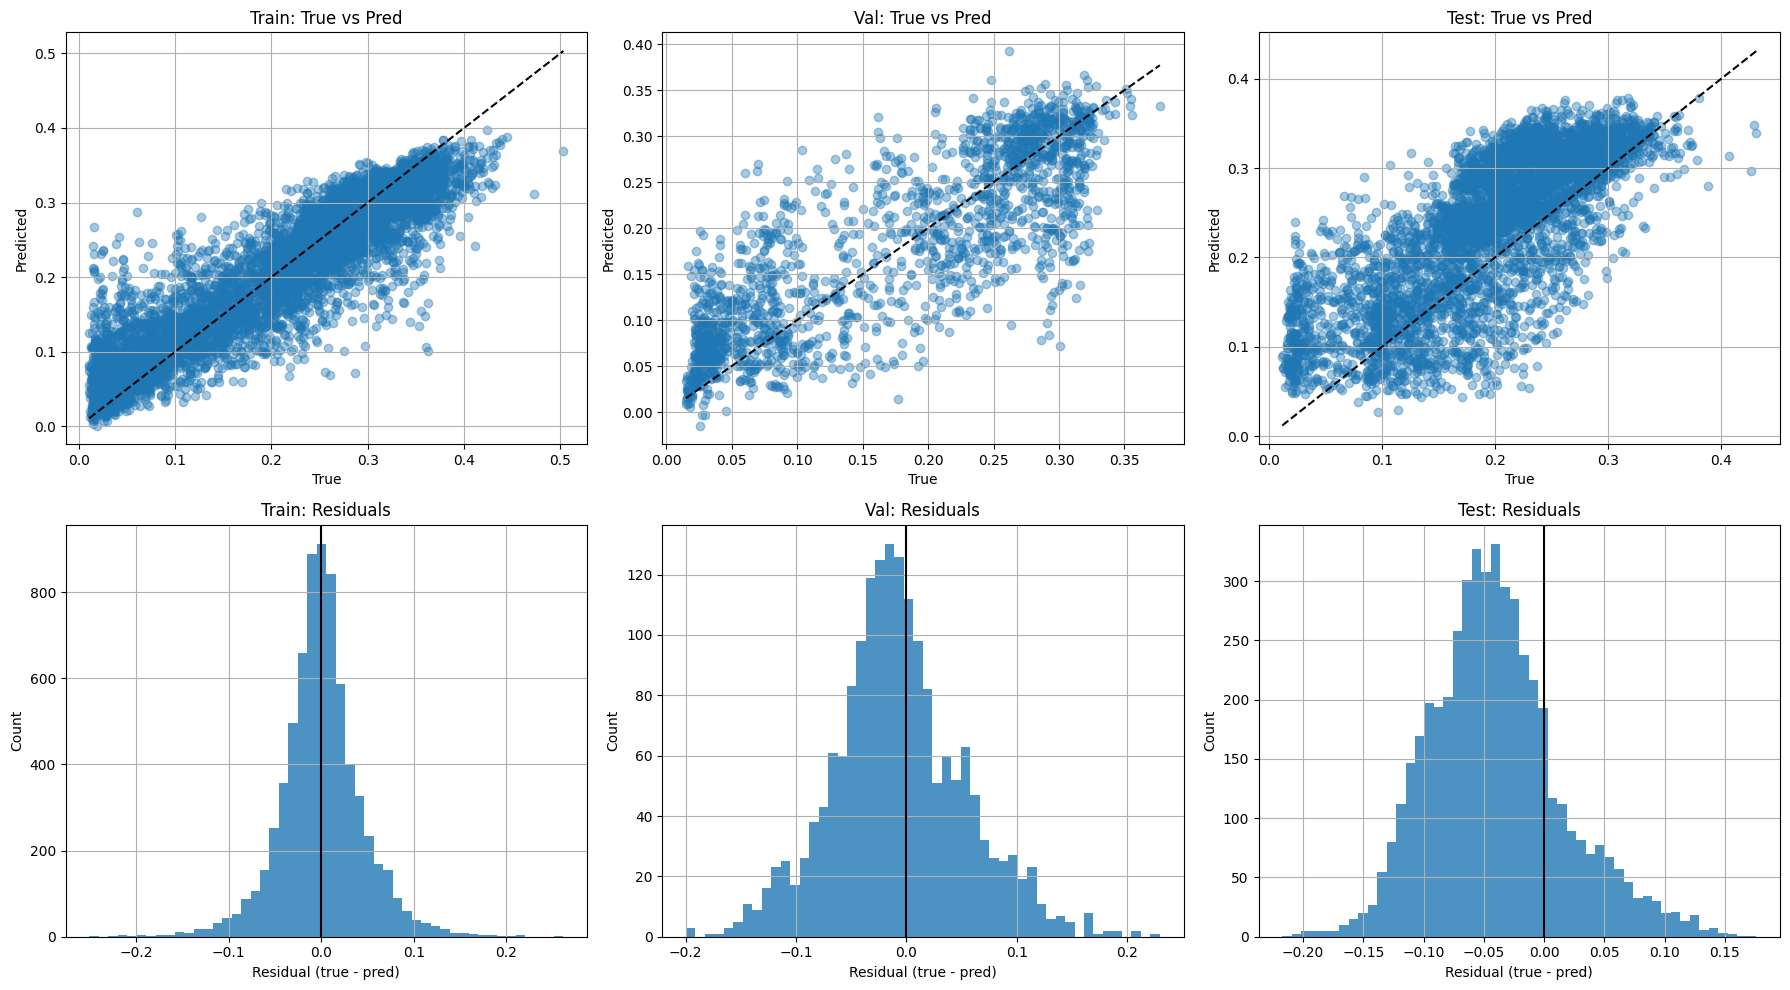
\includegraphics[width=\textwidth]{images/panel.png}
\caption{True vs.\ predicted values (top row) and residual distributions (bottom row) for train, validation, and test splits.}
\end{figure}

\section{Ablation Study}

\subsection{Ablation Methodology}
A leave-one-feature-out ablation was performed to identify features that negatively impact spatial generalization.

\subsection{Key Ablation Results}
The v1.2 baseline, with calendar and atmospheric shortcut features removed, achieved the best balance of error, explained variance, and bias. Further feature removals generally degraded performance.

\subsection{Interpretation}
These results suggest that earlier improvements stem from reducing shortcut learning rather than from increased model complexity.

\section{Discussion}

\subsection{Spatial Generalization Behavior}
Compared to earlier baselines, MDR-TS v1.2 generalizes more reliably to an unseen station, though some bias remains.

\subsection{Role of Surface vs.\ Atmospheric Features}
Surface-sensitive features such as SAR backscatter and vegetation indices appear more transferable across stations than atmospheric variables.

\subsection{Remaining Failure Modes}
The remaining errors are consistent with missing temporal memory and limited spatial diversity in the dataset.

\section{Limitations}

\begin{itemize}
\item Only three stations available
\item Single geographic region
\item No explicit temporal memory features
\item No spatially explicit modeling
\end{itemize}

\section{Future Work}

\subsection{Temporal Memory Features}
Future versions will incorporate precipitation memory features such as API or days since rain.

\subsection{Spatial-Resolution Integration}
The model will be extended using multi-resolution spatial features produced by parallel project work.

\subsection{Dataset Expansion}
Increasing the number of stations will be critical for stronger conclusions about spatial generalization.

\section{Reproducibility and Artifacts}

\subsection{Model Configuration}
\begin{verbatim}
n_estimators = 500
max_depth = 5
learning_rate = 0.05
subsample = 0.8
colsample_bytree = 0.8
reg_lambda = 1.0
random_state = 42
\end{verbatim}

\subsection{Artifacts}
All metrics, figures, and trained models are saved to ensure reproducibility.

\section{Supplemental Plots}

\begin{figure}[H]
\centering
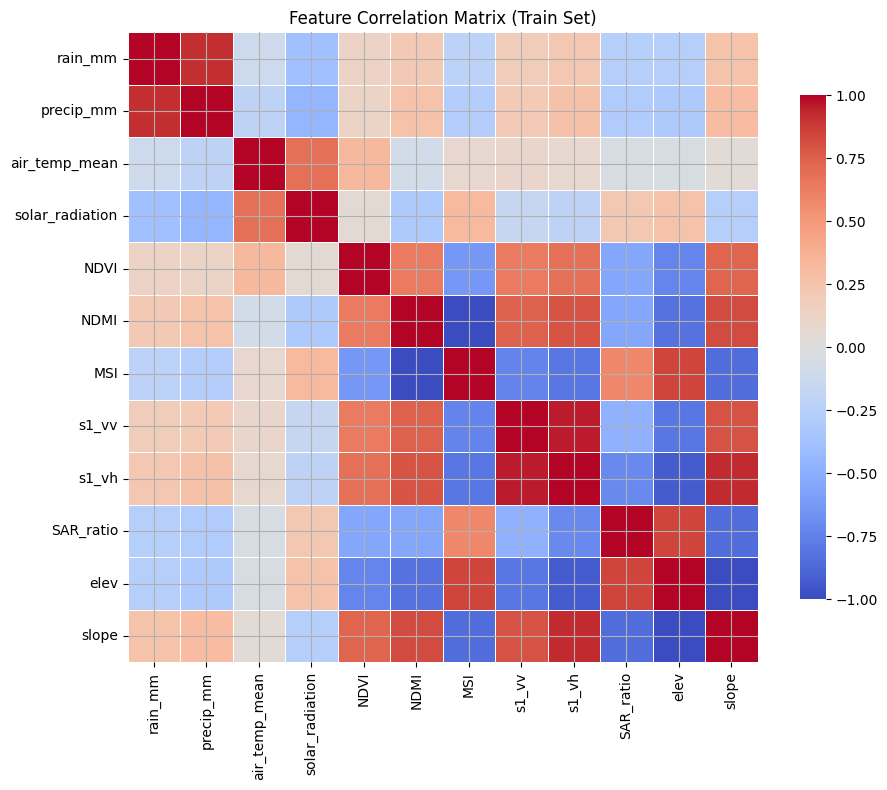
\includegraphics[width=\textwidth]{images/corr_matrix.png}
\caption{Feature correlation matrix for all input variables used in MDR-TS v1.2.}
\end{figure}

\begin{figure}[H]
\centering
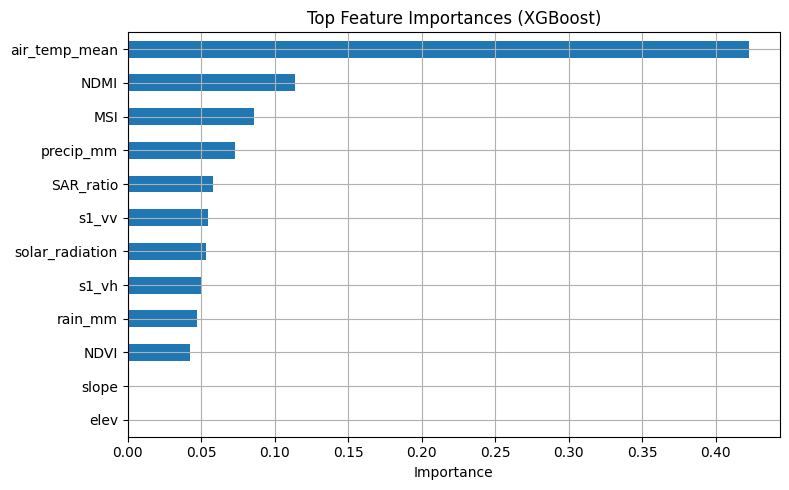
\includegraphics[width=\textwidth]{images/importances.png}
\caption{Feature importance scores from the XGBoost model (v1.2).}
\end{figure}

\begin{figure}[H]
\centering
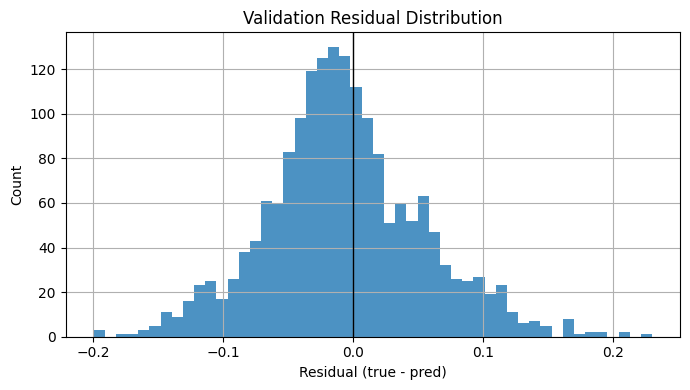
\includegraphics[width=\textwidth]{images/val_residuals_distro.png}
\caption{Validation set: residual distribution.}
\end{figure}

\begin{figure}[H]
\centering
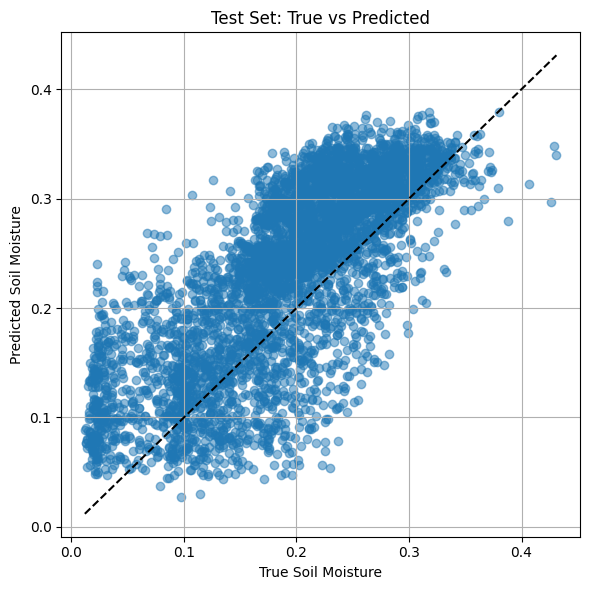
\includegraphics[width=\textwidth]{images/test_true_vs_pred.png}
\caption{Test set: true vs.\ predicted soil moisture values for the held-out station.}
\end{figure}

\begin{figure}[H]
\centering
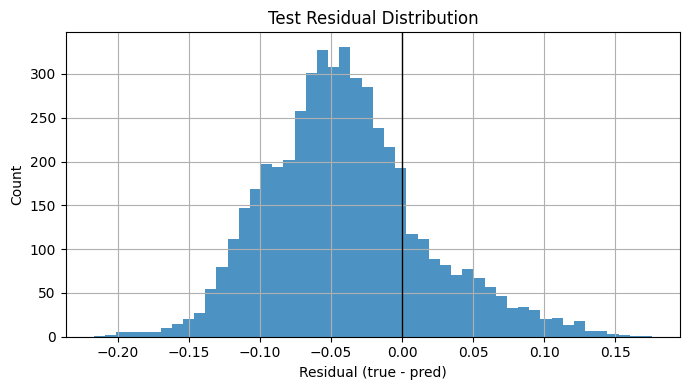
\includegraphics[width=\textwidth]{images/test_residuals_distro.png}
\caption{Test set: residual distribution for the held-out station.}
\end{figure}

\begin{figure}[H]
\centering
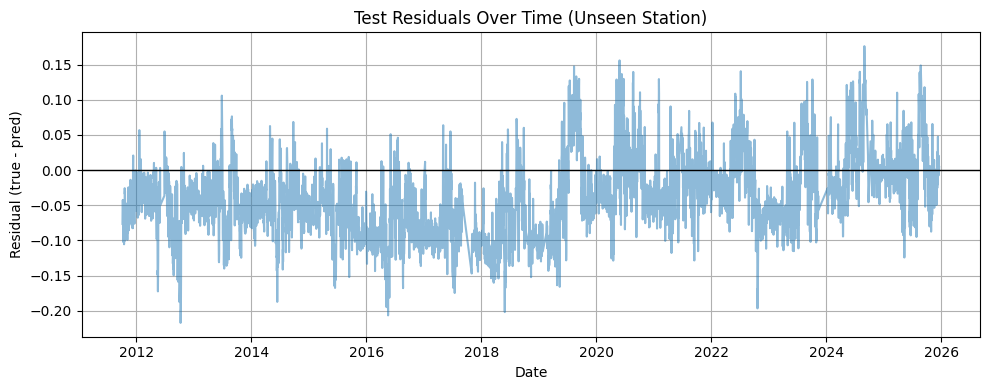
\includegraphics[width=\textwidth]{images/test_residuals.png}
\caption{Test set: residuals plotted over time.}
\end{figure}

\section{Conclusion}

MDR-TS v1.2 provides a clean and interpretable baseline for station-generalized soil moisture prediction and sets a solid foundation for future feature and spatial extensions.

\end{document}